\documentclass[sigconf]{acmart}

% Remove ACM boilerplate, fake DOI, and copyright box
\settopmatter{printacmref=false}
\renewcommand\footnotetextcopyrightpermission[1]{}
\pagestyle{plain}

\usepackage{tikz}
\usepackage{hyperref}
\hypersetup{
    colorlinks=true,
    linkcolor=blue,
    filecolor=magenta,      
    urlcolor=cyan,
}
\usetikzlibrary{trees, shapes.geometric, positioning, fit, calc, backgrounds}

\begin{document}

\title{Which Condition Fits? Multi-Label Diagnosis with Supporting Evidence from Symptom Description}


\author{Niyaaz Baines, Eduardo Kallina de Paula, Thiago Vasconcelos Pinheiro Lopes, Priyanshkumar Ghanshyambhai Patel}
\affiliation{\institution{University of Victoria}}
\email{nbaines@uvic.ca, ekallinadepaula@uvic.ca, thiagovplopes@uvic.ca, priyanshkumarghansh1@uvic.ca}

\begin{abstract}
Symptom overlap among ADHD, anxiety, and depression makes accurate diagnosis difficult, yet most computational models use single-label classification. This project proposes multi-label text classification with verifiable rationale extraction over self-reported symptom descriptions, highlighting the phrases that support each diagnosis. We review prior approaches grouped by the data they use as evidence (conversational, sensor, clinical, and text-based) and position our project among them. Repository: \href{https://github.com/eduardokdp/Data-Mining-Diagnosis}{click here}
\end{abstract}

\keywords{Mental health, text classification, multi-label classification, rationale extraction}

\maketitle

\section{Background and Related Work}

\subsection{Introduction}
Several approaches have been used to address this problem, including natural language processing with conversational analysis, multimodal biomarkers with sensor analysis, machine learning on structured clinical data, and text-based analysis of self-reported symptoms. Conversational analysis uses scripted dialogue trees built on diagnostic criteria to screen for disorders during patient conversations \cite{philip2017virtual}. Sensor analysis examines video footage of patients, paying close attention to eye movement and facial expressions, and combines this with audio recordings to detect signs of depression and related distress \cite{alghowinem2013eye, cummins2015review, gratch2014distress}. Machine learning on structured clinical data applies models ranging from random forests to neural networks to predict the likelihood of a diagnosis and to identify patterns associated with certain mental health conditions \cite{tate2020predicting}.

These approaches differ from ours mainly in the data they rely on. Sensor analysis uses video footage and eye tracking, whereas our method uses only text. Conversational analysis asks structured diagnostic questions, whereas we analyze symptom descriptions written in the person's own words. Structured clinical data approaches draw on a patient's medical records to support a diagnosis, whereas our method relies only on self-reported text.

All three of these approaches have various strengths and limitations. Conversational agents follow diagnostic criteria but miss milder cases; sensors yield objective markers but rely on small, non-standardized corpora; and clinical-record models scale to large cohorts but raise many false alarms (Section 1.4).

\begin{figure}[t]
\centering
\resizebox{\linewidth}{!}{%
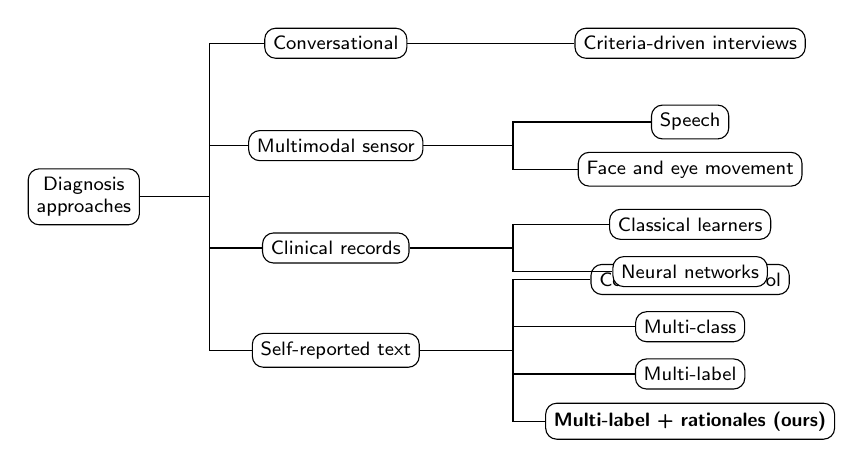
\begin{tikzpicture}[
  edge from parent fork right,
  grow=right,
  level 1/.style={sibling distance=1.3cm, level distance=3.2cm},
  level 2/.style={sibling distance=0.6cm, level distance=4.5cm},
  every node/.style={draw, rounded corners, font=\scriptsize\sffamily, align=center, fill=white, inner sep=3pt},
  edge from parent/.style={draw, -}
]
\node {Diagnosis \\ approaches}
  child { node {Self-reported text}
    child { node[font=\scriptsize\sffamily\bfseries] {Multi-label + rationales (ours)} }
    child { node {Multi-label} }
    child { node {Multi-class} }
    child { node {Condition vs. control} }
  }
  child { node {Clinical records}
    child { node {Neural networks} }
    child { node {Classical learners} }
  }
  child { node {Multimodal sensor}
    child { node {Face and eye movement} }
    child { node {Speech} }
  }
  child { node {Conversational}
    child { node {Criteria-driven interviews} }
  };
\end{tikzpicture}
}
\caption{Hierarchy of prior work: input data (level 1), then dialogue design, modality, learner, or label structure (level 2).}
\label{fig:hierarchy}
\end{figure}

\subsection{History}
The challenge of classifying mental illness predates computing by well over a century. Nineteenth-century psychiatrists relied on inconsistent disease categories until German psychiatrist Emil Kraepelin introduced a more systematic approach to classification in 1899 \cite{kawa2012brief, kraepelin1899psychiatrie}. His approach distinguished conditions such as dementia praecox from manic-depressive illness based on the course and development of symptoms rather than their surface presentation alone. These developments resurfaced in DSM-III (1980), whose neo-Kraepelinian design replaced psychodynamic categories with explicit operational criteria for each disorder \cite{kawa2012brief}. Language also became a measurable signal: depressed students used more first-person singular pronouns and negative-emotion words in expressive writing \cite{rude2004language}, and a decade later self-reported diagnoses on Twitter supplied labels for depression and PTSD classifiers \cite{coppersmith2015clpsych}; by 2022, social-media posts supplied the data for 81\% of 399 reviewed studies \cite{zhang2022natural}.

\subsection{Hierarchy}
We organize prior work by the input data used as diagnostic evidence, which gives four branches (Figure 1): conversational agents, multimodal sensors, structured clinical records, and self-reported text. Sensor work divides by modality (speech versus face and eye movement) and clinical-record work by learner (classical versus neural). Text-based work, the branch closest to ours, divides by label structure: one condition against healthy controls, one of several conditions (multi-class), or several conditions at once (multi-label).

\subsection{Comparative Analysis}
Philip et al. \cite{philip2017virtual} drove a virtual interviewer with a DSM-5 decision tree, reaching 93\% specificity but only 49\% sensitivity, lower still for milder cases. Sensor work adds nonverbal signals: DAIC \cite{gratch2014distress} records interview audio and video alongside questionnaire responses, and speech and eye-movement features \cite{alghowinem2013eye, cummins2015review} give objective markers, although corpora are small and collection protocols are not standardized. Clinical-record models scale instead: Tate et al. \cite{tate2020predicting} reached an AUC of 0.74 for 7,638 adolescents from register and parent-questionnaire data, yet a 15\% positive predictive value limits screening use. 

\begin{figure}[t]
\centering
\begin{tikzpicture}[scale=0.8, every node/.style={font=\scriptsize}]
  \begin{scope}
    \clip (1.5, 0) circle (1.8cm);
    \fill[gray!30] (-1.5, 0) circle (1.8cm) (0, -2.2) circle (1.8cm) (-5,-5) rectangle (5,5);
  \end{scope}
  
  \draw (-1.2, 0) circle (1.8cm);
  \draw (1.2, 0) circle (1.8cm);
  \draw (0, -1.8) circle (1.8cm);
  
  \node[align=center] at (-1.5, 0.5) {[3, 17] \\ [7, 12]};
  \node[align=center] at (1.1, 0.5) {[2, 15]};
  \node[align=center] at (0, -2.5) {[5, 11]};
  \node[align=center, font=\scriptsize\bfseries] at (0, -0.6) {ours};
  \filldraw[black] (-0.3, -0.6) circle (0.8pt);
  
  \node[align=center] at (-2.8, 1.8) {Mental-health text};
  \node[align=center] at (2.8, 1.8) {Multi-label diagnosis};
  \node[align=center] at (0, -4.0) {Extractive rationales};
\end{tikzpicture}
\caption{Positioning by three properties (numbers are references). Only our project combines all three; gray regions are outside our scope.}
\label{fig:venn}
\end{figure}

Text-based methods moved from word counts \cite{rude2004language} to neural encoders: a CNN sorted Reddit posts into 11 themes with 71\% weighted accuracy \cite{gkotsis2017characterisation}, and RoBERTa assigned posts to one of five conditions or none \cite{murarka2021classification}, but both assign one label per post. Multi-label prediction is rarer: SMHD \cite{cohan2018smhd} added a user-level multi-label baseline over nine conditions, and Souza et al. \cite{souza2021deep} modeled depression-anxiety comorbidity directly (exact-match ratio 0.47), yet their best ensemble dropped the comorbidity classifiers. Explanations developed separately: extractive rationales select the input spans behind a prediction \cite{lei2016rationalizing} and can be scored for faithfulness and human agreement \cite{deyoung2020eraser}, whereas MentaLLaMA \cite{yang2024mentallama} generates free-text explanations that need not quote the user's words. Table 1 summarizes these trade-offs; Figure 2 shows that no reviewed method combines all three properties.

\begin{table}[h]
\caption{Strengths and limitations by category.}
\label{tab:comparison}
\resizebox{\linewidth}{!}{%
\begin{tabular}{p{1.5cm}|p{2.5cm}|p{2.5cm}|p{2.5cm}}
\toprule
\textbf{Category} & \textbf{Input data} & \textbf{Strengths} & \textbf{Limitations} \\
\midrule
Conversational & Guided questions in a dialogue & Follows DSM criteria; 93\% specificity. & 49\% sensitivity, lower on milder cases \\
\hline
Sensor & Audio, video, eye movement & Objective, non-invasive markers & Small corpora; no standard protocol \\
\hline
Clinical records & Registers, medical records & Large cohort (AUC 0.74) & 15\% PPV; no external validation \\
\hline
Text-based & Social-media and forum posts & Abundant natural language & Mostly single-label or vs. controls \\
\hline
\textbf{Ours} & \textbf{Self-reported symptom text} & \textbf{Multi-label with phrase evidence} & \textbf{Forum labels not clinically verified} \\
\bottomrule
\end{tabular}%
}
\end{table}

\subsection{Position Your Project}
CLPsych \cite{coppersmith2015clpsych} and SMHD \cite{cohan2018smhd} are the closest benchmarks, but both classify users from their posting histories, mostly against healthy controls (CLPsych adds one depression-versus-PTSD task), and neither shows the evidence behind a prediction. Because ADHD, anxiety, and depression share symptoms such as inattention and restlessness \cite{fu2025adult}, our project builds on multi-label classification \cite{cohan2018smhd, souza2021deep} and extractive rationales \cite{lei2016rationalizing} to separate these commonly confused conditions within a single self-reported description, attaching the supporting phrases to each prediction.

\vspace{2mm}
\noindent \textbf{Contributions.} Niyaaz: history, abstract; Eduardo: introduction, positioning; Thiago: hierarchy, taxonomy; Priyansh: comparative analysis, table.

\begin{thebibliography}{18}

\bibitem{alghowinem2013eye}
Sharifa Alghowinem, Roland Goecke, Michael Wagner, et al. 2013. Eye Movement Analysis for Depression Detection. In \textit{2013 IEEE International Conference on Image Processing (ICIP)}. 4220--4224.

\bibitem{cohan2018smhd}
Arman Cohan, Bart Desmet, Andrew Yates, et al. 2018. SMHD: A Large-Scale Resource for Exploring Online Language Usage for Multiple Mental Health Conditions. In \textit{Proceedings of the 27th International Conference on Computational Linguistics (COLING)}. 1485--1497.

\bibitem{coppersmith2015clpsych}
Glen Coppersmith, Mark Dredze, Craig Harman, et al. 2015. CLPsych 2015 Shared Task: Depression and PTSD on Twitter. In \textit{Proceedings of the 2nd Workshop on Computational Linguistics and Clinical Psychology (CL Psych)}. 31--39.

\bibitem{cummins2015review}
Nicholas Cummins, Stefan Scherer, Jarek Krajewski, et al. 2015. A Review of Depression and Suicide Risk Assessment Using Speech Analysis. \textit{Speech Communication} 71 (2015), 10--49.

\bibitem{deyoung2020eraser}
Jay DeYoung, Sarthak Jain, Nazneen Fatema Rajani, et al. 2020. ERASER: A Benchmark to Evaluate Rationalized NLP Models. In \textit{Proceedings of the 58th Annual Meeting of the Association for Computational Linguistics}. 4443--4458.

\bibitem{fu2025adult}
Xinyu Fu, Weige Wu, Yuru Wu, et al. 2025. Adult ADHD and Comorbid Anxiety and Depressive Disorders: A Review of Etiology and Treatment. \textit{Frontiers in Psychiatry} 16 (2025), 1597559.

\bibitem{gkotsis2017characterisation}
George Gkotsis, Anika Oellrich, Sumithra Velupillai, et al. 2017. Characterisation of Mental Health Conditions in Social Media Using Informed Deep Learning. \textit{Scientific Reports} 7 (2017), 45141.

\bibitem{gratch2014distress}
Jonathan Gratch, Ron Artstein, Gale Lucas, et al. 2014. The Distress Analysis Interview Corpus of Human and Computer Interviews. In \textit{Proceedings of the 9th International Conference on Language Resources and Evaluation (LREC)}. 3123--3128.

\bibitem{kawa2012brief}
Shadia Kawa and James Giordano. 2012. A Brief Historicity of the Diagnostic and Statistical Manual of Mental Disorders: Issues and Implications for the Future of Psychiatric Canon and Practice. \textit{Philosophy, Ethics, and Humanities in Medicine} 7 (2012), 2.

\bibitem{kraepelin1899psychiatrie}
Emil Kraepelin. 1899. \textit{Psychiatrie: Ein Lehrbuch für Studierende und Ärzte} (6th ed.). Johann Ambrosius Barth, Leipzig.

\bibitem{lei2016rationalizing}
Tao Lei, Regina Barzilay, and Tommi Jaakkola. 2016. Rationalizing Neural Predictions. In \textit{Proceedings of the 2016 Conference on Empirical Methods in Natural Language Processing}. 107--117.

\bibitem{murarka2021classification}
Ankit Murarka, Balaji Radhakrishnan, and Sushma Ravichandran. 2021. Classification of Mental Illnesses on Social Media Using RoBERTa. In \textit{Proceedings of the 12th International Workshop on Health Text Mining and Information Analysis (LOUHI)}. 59--68.

\bibitem{philip2017virtual}
Pierre Philip, Jean-Arthur Micoulaud-Franchi, Patricia Sagaspe, et al. 2017. Virtual Human as a New Diagnostic Tool, a Proof of Concept Study in the Field of Major Depressive Disorders. \textit{Scientific Reports} 7 (2017), 42656.

\bibitem{rude2004language}
Stephanie Rude, Eva-Maria Gortner, and James Pennebaker. 2004. Language Use of Depressed and Depression-Vulnerable College Students. \textit{Cognition and Emotion} 18, 8 (2004), 1121--1133.

\bibitem{souza2021deep}
Vanessa Souza, Jéferson Nobre, and Karin Becker. 2021. A Deep Learning Ensemble to Classify Anxiety, Depression, and their Comorbidity from Texts of Social Networks. \textit{Journal of Information and Data Management} 12, 3 (2021).

\bibitem{tate2020predicting}
Ashley E. Tate, Ryan C. McCabe, Henrik Larsson, et al. 2020. Predicting Mental Health Problems in Adolescence Using Machine Learning Techniques. \textit{PLOS ONE} 15, 4 (2020), e0230389.

\bibitem{yang2024mentallama}
Kailai Yang, Tianlin Zhang, Ziyan Kuang, et al. 2024. MentaLLaMA: Interpretable Mental Health Analysis on Social Media with Large Language Models. In \textit{Proceedings of the ACM Web Conference 2024 (WWW 24)}. 4489--4500.

\bibitem{zhang2022natural}
Tianlin Zhang, Annika M. Schoene, Shaoxiong Ji, and Sophia Ananiadou. 2022. Natural Language Processing Applied to Mental Illness Detection: A Narrative Review. \textit{npj Digital Medicine} 5 (2022), 46.

\end{thebibliography}

\end{document}